\subsection{ESCON 50/5 motor controller}\label{sec:motor_control}
For driving the motors, four ESCON motor drivers of the type 50/5 (part number 438725) have been implemented, see \figref{fig:ESCON505}. 

\begin{figure}[H]
	\centering
		\centering
		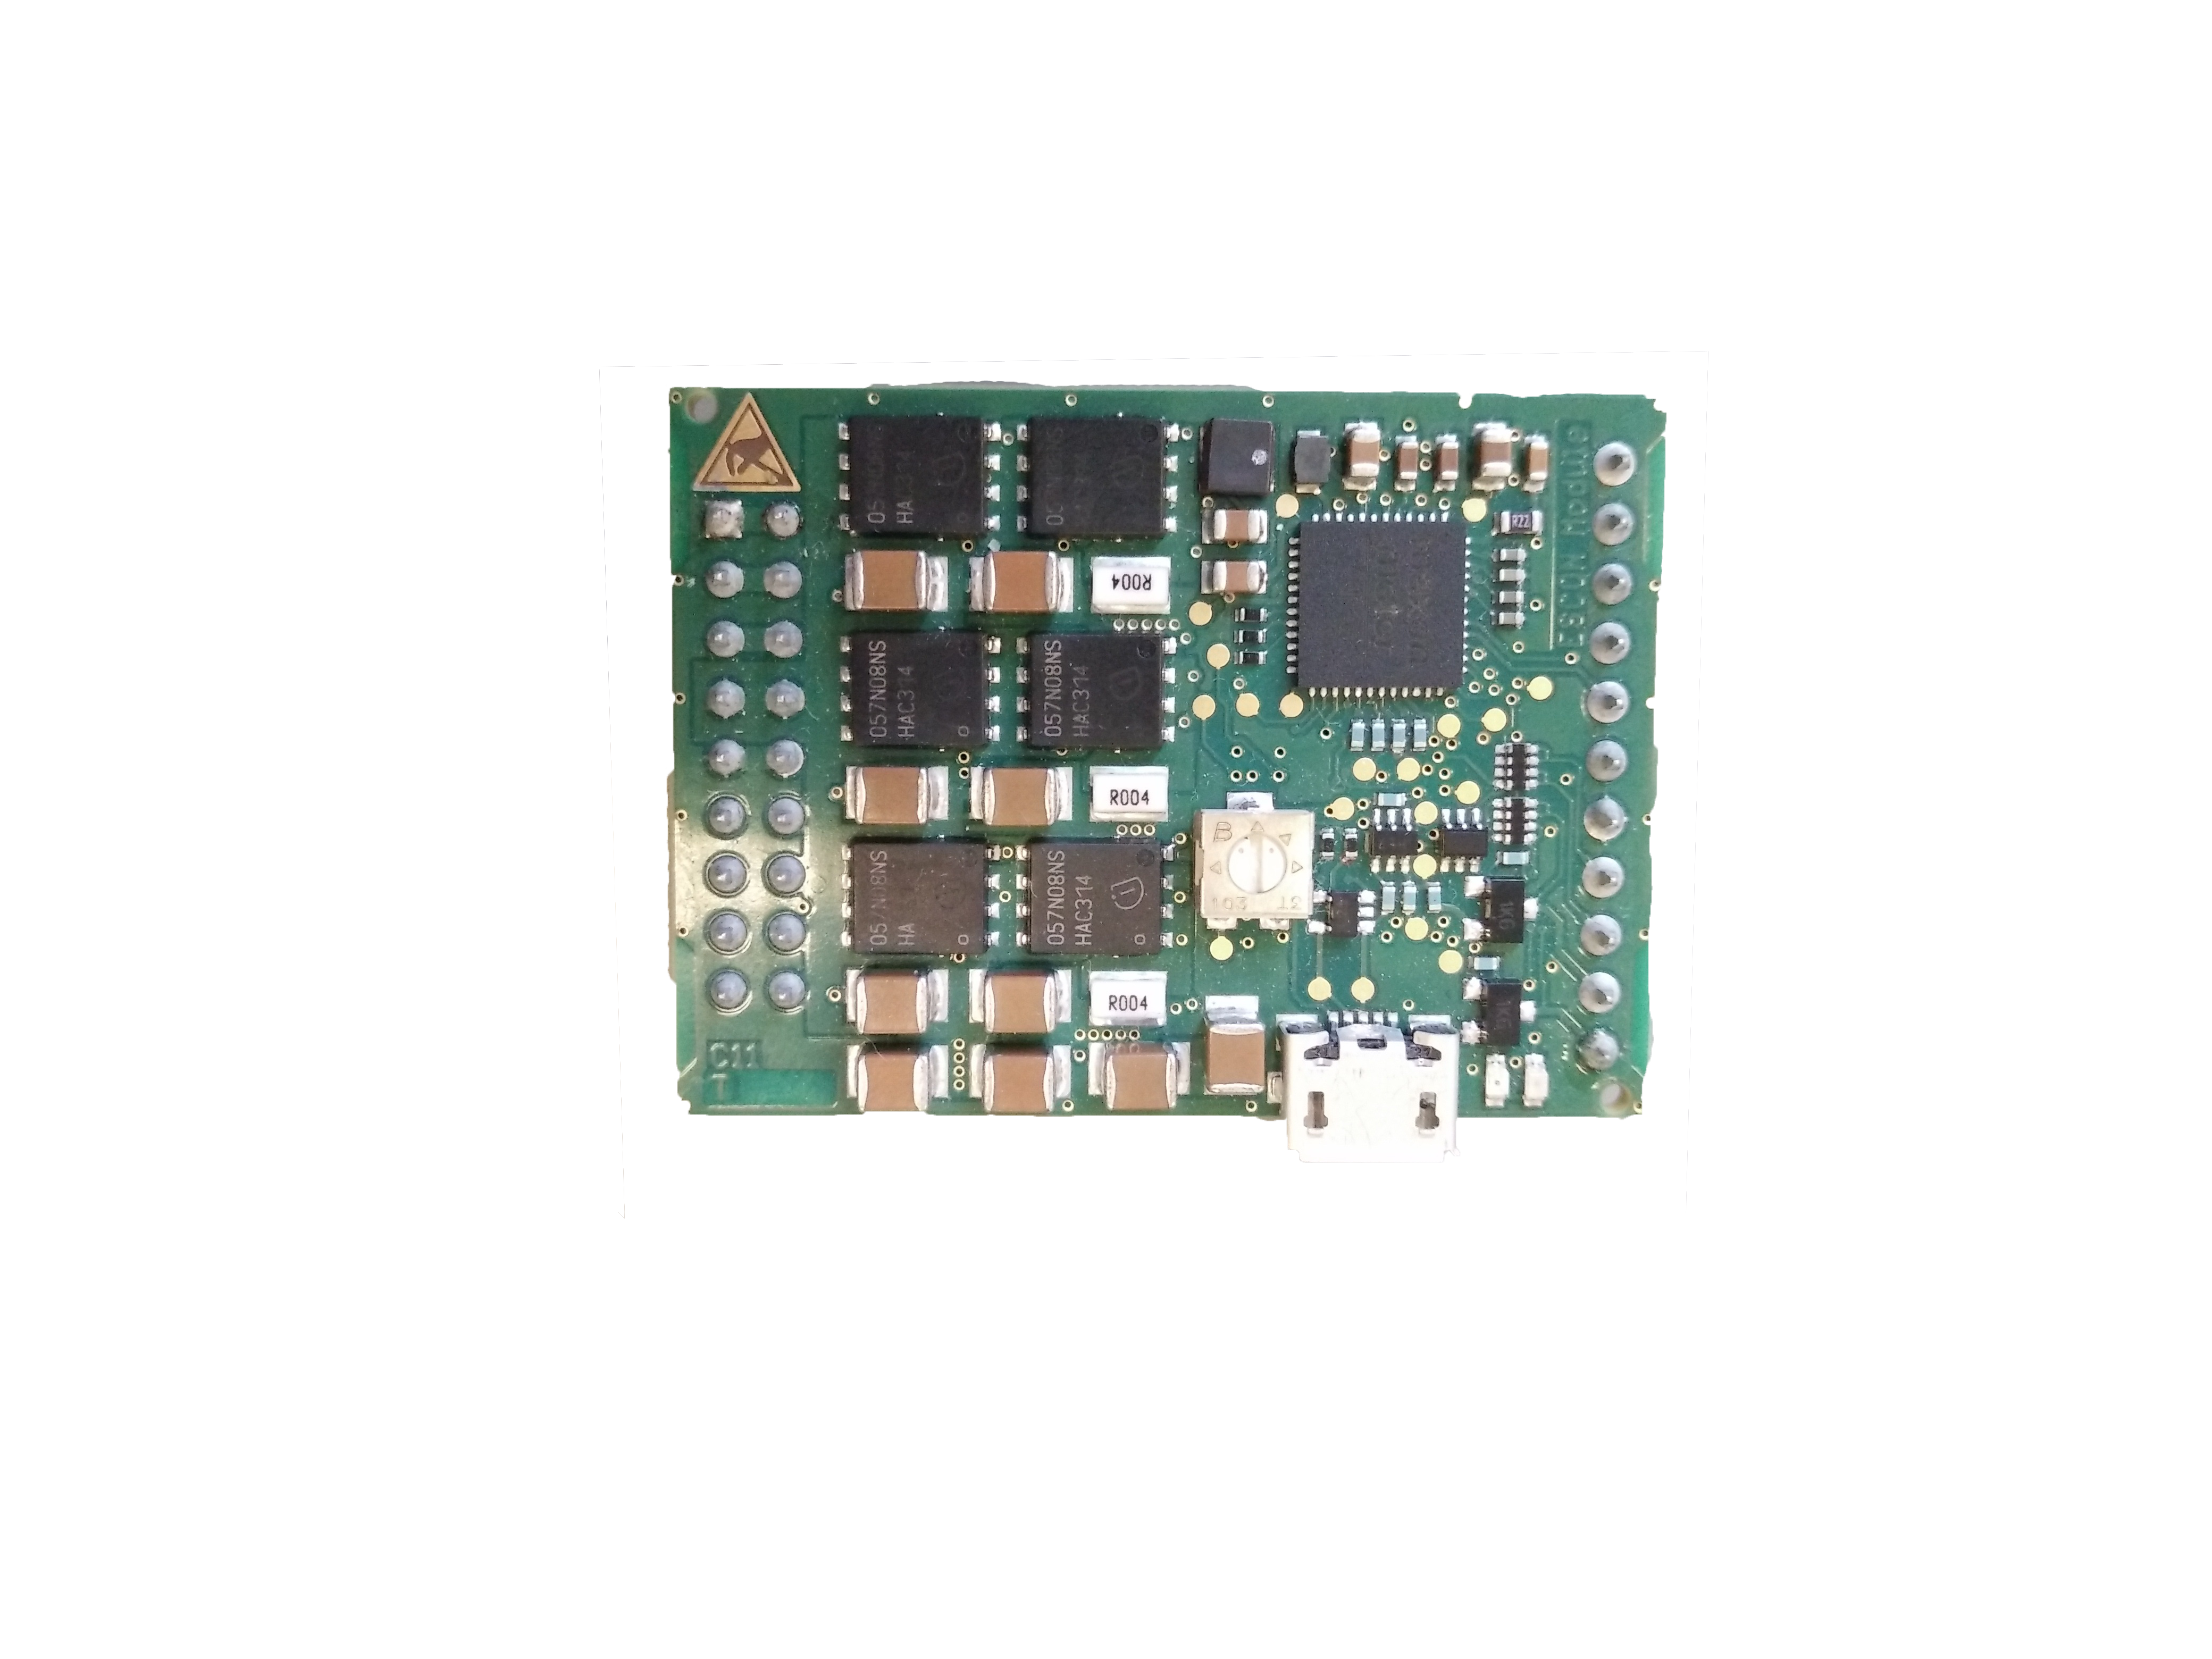
\includegraphics[width=0.7\linewidth]{ESCON505.png}
		\caption{ESCON 50/5 DC motor controller\cite{ESCON_motor_controller}}
		\label{fig:ESCON505}
\end{figure}

These are controllers made for permanent magnet-activated brushed DC motors. They can deliver a power up to 250 Watt for the motor connected to the controller. 

The ESCON 50/5 has three operating modes

\begin{itemize}
\item Current controller
\item Speed controller (open loop)
\item Speed controller (closed loop)
\end{itemize}

The reason we chose speed controller with inner loop current control is explained in \ref{escon_con}.
Each motor hosts an encoder that provides relative angular position information to the FPGA built into the sbRIO board.
The ESCON controllers send the speed and current data of the motor to the sbRIO through analog outputs. 